\chapter{Related Work} 
\label{ch:relatedwork}

As the field of AI has grown, more and more researchers are looking into the extent of the capabilities of AI.  The creation of music with computers has gained increased attention within the last decade, however, this does not mean that these tools have gained popularity among users.  Quite a few of these composers have been developed, but only a very small number of them have seen industry use and almost none of them have been used outside of research or these niche areas in industry.

\vspace{\baselineskip}

The reason for this primarily is that the focus of researchers when creating these tools is how advanced the composer can be and what new ways can AI be employed to create more original music.  Their focus is not at all on how these tools can be made in a way that they might find a larger user base or even a user base at all.  This limits what might come of these technologies now and in the future.

\vspace{\baselineskip}

Setting this aside, however, the researchers that have developed these composers have created some very impressive tools capable of creating very convincing music.  This project aims more to guide the user through the process of composing music.  This is different than a majority of the research projects in this area that focus on creating a composer that can write its own music, but the writing still contains an important discussion of how computers can be used to create music.

\section{AI Powered Composers}
\label{sec:aipoweredcomposers}

The following works discuss several different AI based composers that were created to generate their own music.  For the purpose of this thesis, they will be analyzed for their effectiveness at composing as well as their shortcomings as tools that only have limited usability.  All of these have proven to be effective at creating music, but none of them have shown popularity as music composition tools.

\subsection{FlowComposer}
\label{subsec:flowcomposer}

Of the existing AI composers, FlowComposer is the only one that has seen use in industry \cite{Papadopoulos_2016}.  An album that was recorded consisting of only music created with FlowComposer was released in 2017 \cite{Papadopoulos_2016}.  This is also one of the only tools that has an actual visual user interface and is not strictly accessed through the command line.  It is currently being developed as part of Sony CSL and Flow Machines, but is not available to the public for use \cite{Papadopoulos_2016}.  An audio example of what FlowComposer is capable of producing is available on their website, \url{https://www.flow-machines.com}, but access to the tool itself is not provided \cite{Flow_2018}.

\vspace{\baselineskip}

The French composer Jean-Michel Jarre is using Flow Machines to create an "infinite album" \cite{Savage_2019}.  This is a never ending, constantly evolving piece of music generated by Flow Machines from a large library of musical samples \cite{Savage_2019}.  The album is available in JarreLab's EON app \cite{Jarre_2019}.  The music that you hear is generated in real time and will never be heard again \cite{Jarre_2019}.  A link to download the app can be found here: \url{https://jeanmicheljarre.com}.

\vspace{\baselineskip}

FlowComposer was designed to create new songs automatically in any style or can generate the style based on user provided parameters and input \cite{Papadopoulos_2016}.  This tool is capable of re-harmonization (taking an existing melody and create new harmonies in different styles), variation (taking the melody and introducing variations into the pitch content and rhythm), and rendering (playing back a given score as if it were being performed) \cite{Flow_2018}.

\vspace{\baselineskip}

The musical output of this tool is a lead sheet that is scored for a full band.  The music that FlowComposer produces fits into the category of popular songs (e.g. Pop, Jazz, Rock, R \& B, etc.).  It comes out fully notated and able to be performed or recorded.  It is a very high quality tool and very capable at writing songs, but due to its research based nature, is kept from the public.  It is highly likely also that this tool would be very expensive if it were available to the public.  Maybe in the future, this will be a tool that is made available, but it will doubtfully ever be accessible to the average person due to the potential price.

\subsection{BachProp}
\label{subsec:bachprop}

BachProp is a neural composer algorithm that was created to be able to compose new music in any style \cite{Colombo_2018Com}.  It was trained initially on the chorales of J. S. Bach, but is able to compose in any style when given appropriate training data \cite{Colombo_2018Com}.  The data is fed to the composer through MIDI files which are mathematically normalized before being translated into probability data that the algorithm uses to predict melodic direction and shape \cite{Colombo_2018Com}.

\vspace{\baselineskip}

For the evaluation of BachProp, audiences were asked to rate several string quartets that it composed after it was trained on string quartets by Haydn and Mozart \cite{Colombo_2018Com}.  Based on the results of the surveys, the music was not only well received, but it was also quite convincingly in the appropriate style and character \cite{Colombo_2018Com}.  To hear some of the music that Bach Prop composed, visit: \url{https://sites.google.com/view/bachprop-icml18/}.

\vspace{\baselineskip}

The process of actually performing crowd based musical validation is quite important here.  Rather than the researchers who developed the composer rating the music, they had general audiences perform the reviews to better understand the broad appeal of the music.  In this project, a similar crowd based reviewing of the interface was performed.  Participants individually judged their created music in their own terms so that their personal success was measured to be able to determine if the user interface was able to guide them through the composition process.

\vspace{\baselineskip}

BachProp has also been used and evaluated in the composition of music in a number of other styles \cite{Colombo_2018Gen}.  The method of musical representation used by BachProp has proven to be more effective at capturing and later translating the information from the provided training scores than other algorithmic composers \cite{Colombo_2018Gen}.  By normalizing how the musical data is stored, this tool is able to gather and retain more detail from the score than other composers \cite{Colombo_2018Gen}.  This is what makes BachProp more effective at emulating a given style and producing more convincing musical output \cite{Colombo_2018Gen}.

\vspace{\baselineskip}

In order for the several Python libraries that were used to create the composer to cooperate, the musical data for this project was also represented in a normalized manner.  Like BachProp, the data was represented as MIDI events to provide a standard for communication and output.  This also means that at any step in the composition process the data could be imported into any standard music notation program and used externally to the composer as MIDI is the standard for digital music notation representation and playback.

\vspace{\baselineskip}

The largest shortcoming of BachProp is that it was not designed in a way that can be used without extensive music or computer science knowledge.  This means that is highly unlikely that it would ever be picked up by someone who simply wanted to play around with it or experiment with it.  There is an extensive setup involved and it cannot be used by any simple means.  However, BachProp is able to produce high quality music in any style and not just popular music as FlowComposer does.

\subsection{DeepBach}
\label{subsec:deepbach}

DeepBach is a graphical model for musical composition that is designed to be effective at producing polyphonic music in four part hymn format \cite{Hadjeres_2016}.  This is yet another composer that was trained on the music of J. S. Bach in order to teach it the mechanics of composition and in this case, to teach it chorales specifically \cite{Hadjeres_2016}.  This composer is able to produce convincing Bach chorale style pieces that are driven by user parameters and input \cite{Hadjeres_2016}.  The following are examples of chorals composed by DeepBach.  Below each, is a chordal analysis in slash chord notation.

\pagebreak

It is important to note that examples (a) and (b) were created using the same user input data and parameters.  This shows that there are at least several different possibilities for harmonization and development of the melodic line.  Before the individual examples are discussed, there are some important similarities that are shared between the chorales.

\vspace{\baselineskip}

The first of these is the handling of steps and leaps in each of the voices.  It will later be discussed that it is appropriate to move in step wise motion in the opposite direction after leaping.  In each voice in each example this rule is exactly followed.

\vspace{\baselineskip}

The next similarity is in the cadences at the ends of the chorales.  In both example (a) and (c) we see, in the last three chords, a move from some version of V7 of V, to V, to I.  This is a very typical progression and is resolved correctly in both the soprano and bass voices by stepping and leaping respectively.  In example (b) we have a similar progression, but it does not use V7 of V.

\vspace{\baselineskip}

Another similarity comes in the treatment of the different voices.  The soprano voice, which has the melody, contains much less motion and overall activity as compared to the other voices.  This is good practice in melody composition as the melody should be easy to remember and sing back.

\vspace{\baselineskip}

Yet another similarity can be found with the use of chromaticism in the passing tones and shift between chords.  To provide both harmonic interest and a form of melodic interest within each of the parts, come chromatic motion is used.  When it is used, it is resolved appropriately with stepwise motion.

\pagebreak

\begin{figure}[!htbp]
	\centering
	\caption{Score (a) from Hadjeres's published paper showing DeepBach output \cite{Hadjeres_2016}}
	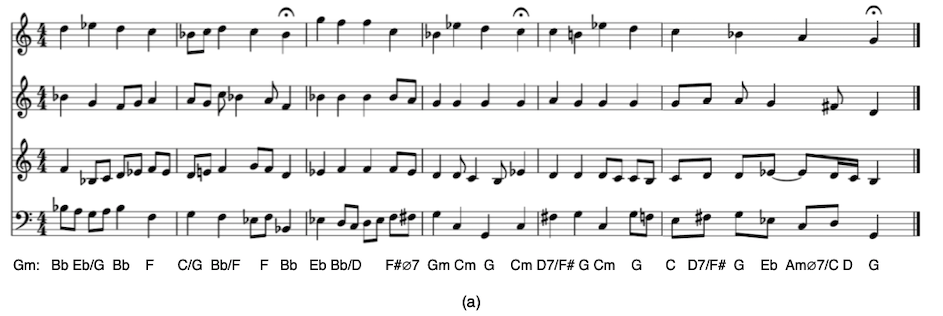
\includegraphics[scale=0.3]{images/deepbachOutputA.png}
\end{figure}

This example (a) is in the key of G Minor.  While it does end in G Major, the presence of B\fl 's and E\fl 's put it in G Minor.  The fact that it ends in G Major is not uncommon however.  It was often the practice to end a chorale in a minor key with the major version of the I chord by raising the third.

\vspace{\baselineskip}

This example in particular uses more chords outside of the normal key material than the other two.  However, the two cadences within the chorale (indicated by the fermatas) are both firmly within G Minor.

\begin{figure}[!htbp]
	\centering
	\caption{Score (b) from Hadjeres's published paper showing DeepBach output \cite{Hadjeres_2016}}
	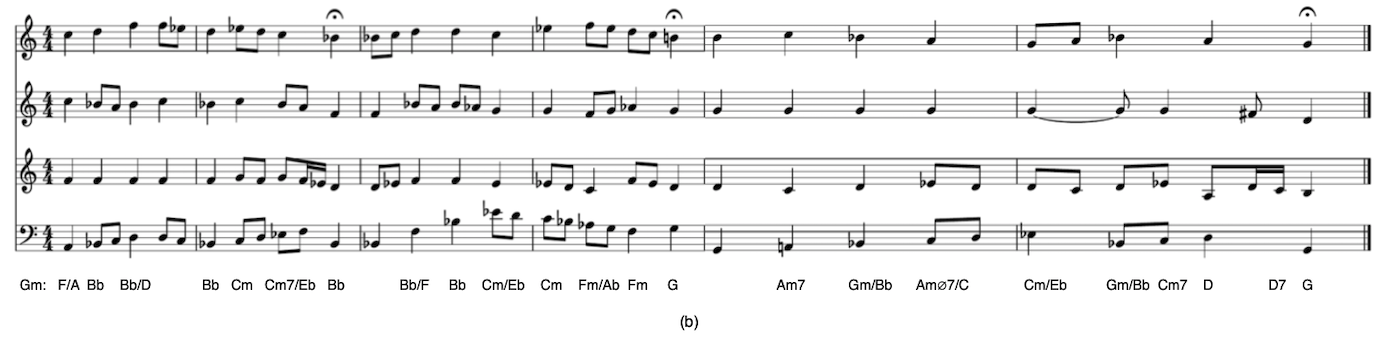
\includegraphics[scale=0.3]{images/deepbachOutputB.png}
\end{figure}

As mentioned previously, this example (b) was made with the same user input data as the previous example.  Also like the first example, this one also ends in the parallel major.  This is not a requirement of this style.  Both examples just happen to leverage this technique.

\vspace{\baselineskip}

This example has some out of key material, but not as much as the first example.  It also moves to the relative major in the second of the two internal cadences instead of only at the end.  While they do share the same metadata, they are distinct in their melodies, progressions, and voice leading.

\pagebreak

\begin{figure}[!htbp]
	\centering
	\caption{Score (c) from Hadjeres's published paper showing DeepBach output \cite{Hadjeres_2016}}
	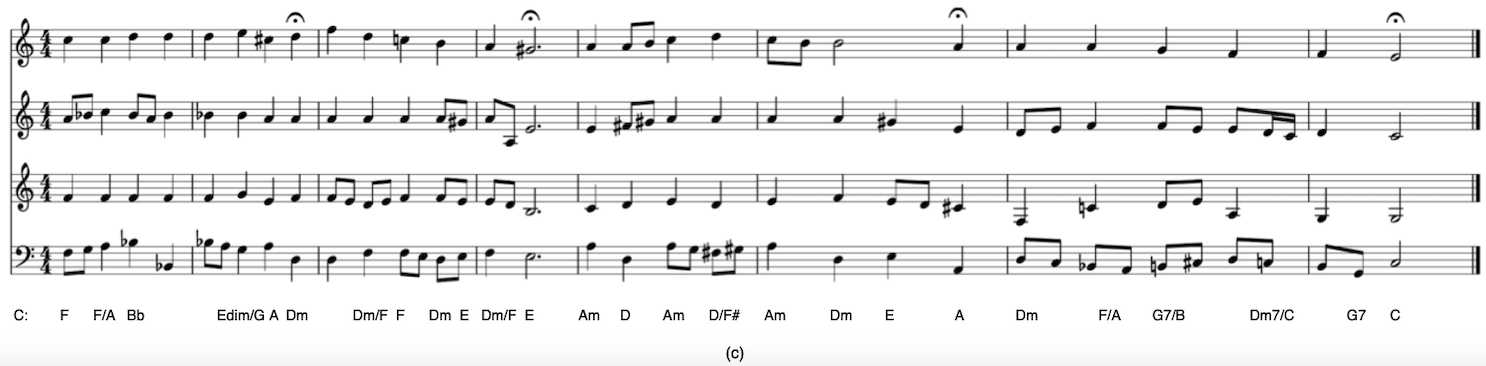
\includegraphics[scale=0.3]{images/deepbachOutputC.png}
\end{figure}

This third example (c) is in C Major.  It also has one more cadence than the other two examples.  Another factor that makes this example different is that there is noticeably more chromatic motion in each of the voice parts.

\vspace{\baselineskip}

While this has more material from outside the key than the second example, it does not have as much as the first.  In this case however, the internal cadences are from outside the key.  They are, however, distantly related as E Major is V of A Major, A Major is V of D Major, D Major is V of G Major, and G Major is V of C Major.  This progression can be seen across the chords at the second two fermatas and final three chords.

\vspace{\baselineskip}

DeepBach does provide integration with the notation program MuseScore \cite{Hadjeres_2016}.  This means that there is a way in which people who are familiar with notation software could use this composer.  While this is better than many of the others, it still requires a fair bit of prior knowledge.  Additionally, this composer is not capable of operating in more than four part chorale style.  The potential uses of this composer are very limited due to this fact.